\documentclass{ximera}
\title{Rational Functions with Awful Questions}
\begin{abstract}
\end{abstract}
\begin{document}
\maketitle
\section{Introduction}
\begin{dialogue}
\item[James] Hey guys, I slept through class yesterday... could you fill me in on what a rational function is?
\item[Julia] See, class didn't make a lot of sense to me because I was thinking, ``Functions can be rational?''
\item[Dylan] They don't mean rational like me or you, Julia! It means \textit{the function can be represented as a fraction where the numerator and denominator are both polynomials}.
\item[Julia and James] Oh!
\item[Dylan] Rational functions are pretty neat, because they can have two different types of discontinuities!
\item[Altogether] LET'S DIVE IN!
\end{dialogue}
\section{Guided Example}
Consider the function $f(x)=\frac{(x-2)(x+4)}{(x-3)(x+3)(x+4)}$
\begin{image}
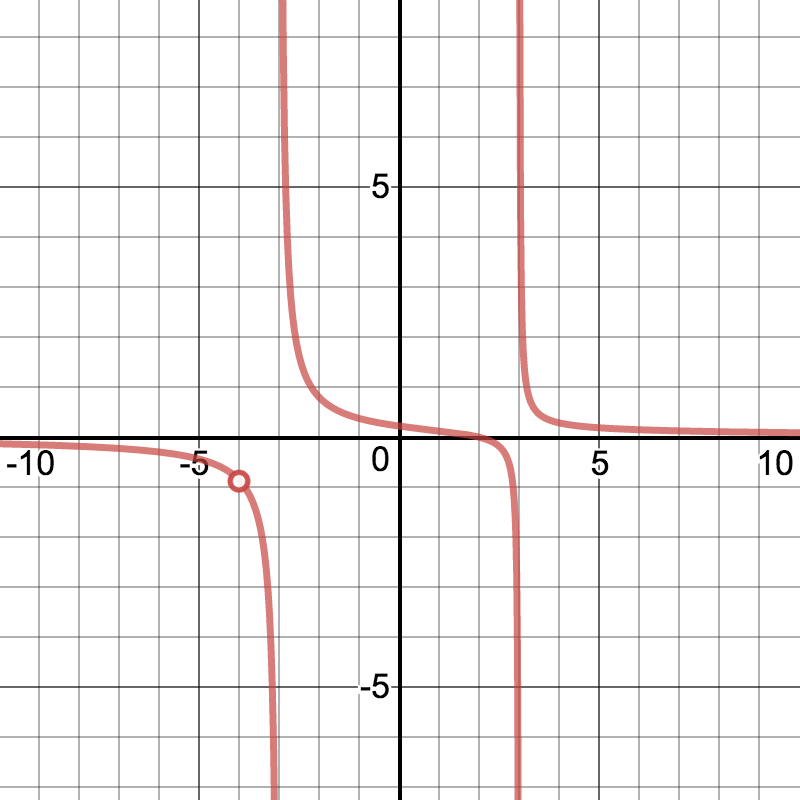
\includegraphics{discontinuityGraph}
\end{image}

\begin{question}
Describe the graph. What strange things do you notice?
\begin{freeResponse}
\end{freeResponse}
\end{question}
The "hole" present in the graph is called a \textbf{removable discontinuity}.

The curve which goes vertical is called a \textbf{vertical asymptote}, another type of discontinuity.

\section{On Your Own}
Depending on the CAS you use, you may need to research how to show discontinuities in a graph. To do this, simply Google "\textit{CAS} show discontinuities", where \textit{CAS} is the name of whatever CAS you are using. At the time this document was written, Desmos did not include discontinuities. If you are unable to display removable discontinuities, you will need to find them by hand.

Find and report the locations of discontinuities in the following functions:

\begin{question}
$a(x) = \dfrac{x^2+1}{x-2}$
\[
\graph{\frac{x^2+1}{x-2}}
\]
\begin{selectAll}
\choice[correct]{$x=2$}
\choice{$x=-1$}
\choice{$x=1$}
\choice{$x=0$}
\end{selectAll}

$b(x) = \dfrac{x^2-5x+7}{x^2-x-6}$

$\answer{}$

$c(x) = \dfrac{x^2-x}{x}$

$\answer{}$

$d(x) = \dfrac{x^2-5x+7}{x^3-6x^2+8x-3}$

$\answer{}$

$f(x) = \dfrac{2x^2+5}{x^2-25}$

$\answer{}$

$g(x) = \dfrac{x^3-x^2-15x-9}{x+3}$

$\answer{}$

$h(x) = \dfrac{1}{3x^2-x}$

$\answer{}$
\end{question}
\begin{question}
How can you tell if a rational function has a vertical asymptote or a removable discontinuity?
\begin{multipleChoice}
\choice[correct]{Vertical asymptotes occur where only the denominator approaches zero, and removable discontinuities occur where both the numerator and denominator approach zero.}
\choice{Vertical asymptotes occur where only the numerator approaches zero, and removable discontinuities occur where both the numerator and denominator approach zero.}
\choice{Vertical asymptotes occur where both the numerator and denominator approach zero, and removable discontinuities occurwhere only the denominator approaches zero.}
\choice{Vertical asymptotes occur where only the numerator approaches zero, and removable discontinuities occurwhere only the denominator approaches zero.}
\end{multipleChoice}
\end{question}

\section{In Summary}
\begin{dialogue}
\item[James] These functions are pretty neat! What were they called again?
\item[Dylan] They're called \textbf{rational functions}, \textit{fractions where the numerator and denominator are both polynomials}!
\item[Julia] So, when exactly does a \textbf{vertical asymptote} occur?
\item[James] I know this one! \textbf{Vertical asymptotes} \textit{occur at points where the denominator of the function will be zero, but the numerator is non-zero}!
\item[Julia] That makes sense! But when do removable discontinuities occur then?
\item[Dylan] \textbf{Removable discontinuities} \textit{occur where the numerator and denominator are both zero}.
\end{dialogue}
\end{document}
